\documentclass[a4paper,12pt]{article}
\usepackage{latexsym}
\usepackage{graphicx}
\usepackage{epsfig}
\usepackage{float}
\usepackage{natbib}
\usepackage{listings}
\usepackage[skip=0pt]{caption}
\graphicspath{{./}}
\DeclareGraphicsExtensions{.eps}
%\setlength\abovecaptionskip{-5pt}
\author{Howard Kinsman}
\title{MSc Project - Modelling a Double Barred Galaxy as a Double Binary}
\begin{document}
\maketitle
\begin{abstract}
TODO
\end{abstract}
{\bf Keywords:} TODO
\section{Introduction}
The aim of this project was to create a simple model of a double barred galaxy using a double binary.

\section{Methods}
Fortran 90 was selected as the language of choice in order to avoid the fixed line limitations of Fortran 77.
The model was created using OdeInt from Numerical Recipes. I first converted OdeInt to Fortran 90 for this purpose.
Please see the Compilers subsection for a few notes on compilers - may or may not be relevant to the project.
\newline
The classical equations of motion for an n-body problem are:
\begin{equation}
m_i\mathbf{\ddot{r}}=\sum_{i\neq{j}}\frac{{m_i}{m_j}}{r^3_{ij}}\mathbf{r_{ij}}
\qquad
i=1,2,3...
\end{equation}
where $\mathbf{r_i}=\left(x_i,y_i\right)$ and $\mathbf{r_{ij}}=\mathbf{r_j}-\mathbf{r_i}$. So for a four body problem 
this equation results in the following:
\begin{equation}
\ddot{\mathbf{r_1}}=\frac{m_2\mathbf{r}_{12}}{r^3_{12}}+\frac{m_3\mathbf{r}_{13}}{r^3_{13}}+\frac{m_4\mathbf{r}_{14}}{r^3_{14}}
\end{equation}
\begin{equation}
\ddot{\mathbf{r_2}}=\frac{m_1\mathbf{r}_{21}}{r^3_{21}}+\frac{m_3\mathbf{r}_{23}}{r^3_{23}}+\frac{m_4\mathbf{r}_{24}}{r^3_{24}}
\end{equation}
\begin{equation}
\ddot{\mathbf{r_3}}=\frac{m_1\mathbf{r}_{31}}{r^3_{31}}+\frac{m_2\mathbf{r}_{32}}{r^3_{32}}+\frac{m_4\mathbf{r}_{34}}{r^3_{34}}
\end{equation}
\begin{equation}
\ddot{\mathbf{r_4}}=\frac{m_1\mathbf{r}_{41}}{r^3_{41}}+\frac{m_2\mathbf{r}_{42}}{r^3_{42}}+\frac{m_3\mathbf{r}_{43}}{r^3_{43}}
\end{equation}
The above equations were encoded into Fortran. A full code listing is supplied in a separate file.
\subsection{Initial Conditions}
As a starting point both the outer binary and inner binary were placed in circular orbits and tested separately and then combined to ensure a stable
starting point. The inner binary had initially a neglible mass.
The outer binary initial conditions were:
\begin{lstlisting}
m1=.5, m2=.5, x1=-.5, x2=.5, y1=0, y2=0,
vx1=0, vx2=0, vy1=-.5, vy2=.5
\end{lstlisting}
and for the inner binary:
\begin{lstlisting}
m3=.001, m4=.001, x3=-.001, x4=.001, y3=0, y4=0, 
vx3=0, vx4=0, vy3=-.5, vy4=.5
\end{lstlisting}
Plots of the two initial binaries are shown in Fig. \ref{fig:outerbinary} and 
\ref{fig:innerbinary}. The scale of the inner binary is so small that it is difficult
to see in GnuPlot.
\begin{figure}[H]
\centering
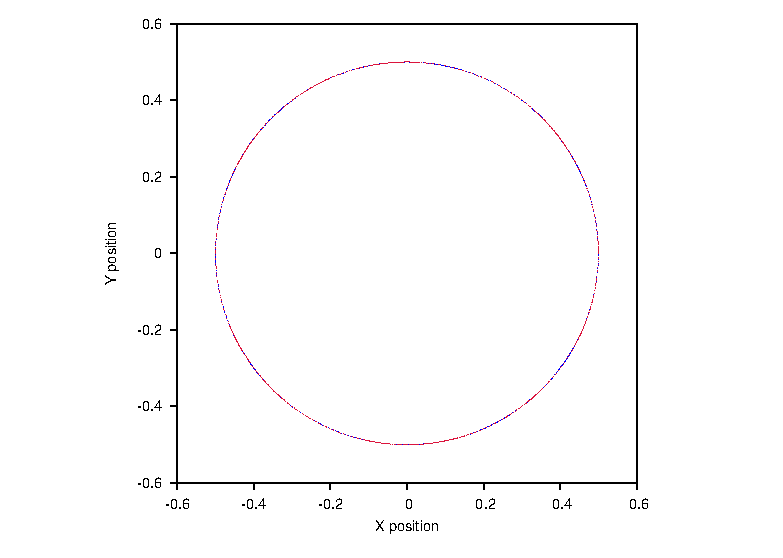
\includegraphics[width=.9\textwidth]{./2016results/outerbinary/Orbit.eps}
\caption{Outer Binary}
\label{fig:outerbinary}
\end{figure}
\begin{figure}[H]
\centering
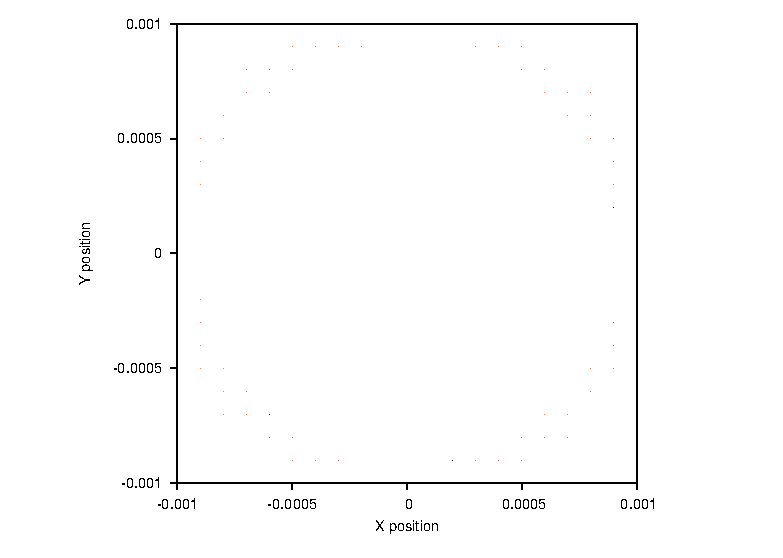
\includegraphics[width=.9\textwidth]{./2016results/innerbinary/Orbit.eps}
\caption{Inner Binary}
\label{fig:innerbinary}
\end{figure}
I then proceeded to perturb the system by gradually increasing the mass of the inner binary. As the system became unstable I componensated for
the increasing mass of the inner binary by increasing the velocity of the outer binary and also decreasing the velocity and increasing the binary 
separation of the inner binary. In many of the configurations the systems were inherently unstable and produced collisions with some 
or all of the bodies being ejected from the system. These were rejected and only 'stable' configurations were considered.
Table \ref{tab:variables} shows the perturbations made to the system - only the variables in this table changed and all the other initial
conditions remained the same.
\begin{table}[ht!]
  \centering
  \caption{Configurations}
  \label{tab:variables}
  \begin{tabular}{ccccccccc}
   Config. & m3 & m4 & vy1 & vy2 & x3 & x4 & vy3 & vy4\\
    \hline
   1 & .001 & .001 & -.5 & .5 & -.001 & .001 & -.5 & .5\\
   2 & .002 & .002 & -.5 & .5 & -.001 & .001 & -.5 & .5\\
   3 & .003 & .003 & -.5 & .5 & -.001 & .001 & -.5 & .5\\
   4 & .004 & .004 & -.5 & .5 & -.004 & .004 & -.5 & .5\\
   5 & .004 & .004 & -.55 & .55 & -.004 & .004 & -.5 & .5\\
   6 & .004 & .004 & -.57 & .57 & -.004 & .004 & -.5 & .5\\
   7 & .005 & .005 & -.58 & .58 & -.005 & .005 & -.3 & .3\\
   8 & .005 & .005 & -.58 & .58 & -.005 & .005 & -.4 & .4\\
   9 & .005 & .005 & -.58 & .58 & -.005 & .005 & -.35 & .35\\
   10 & .006 & .006 & -.6 & .6 & -.006 & .006 & -.3 & .3\\
   11 & .025 & .025 & -.65 & .65 & -.02 & .02 & -.5 & .5\\
   12 & .025 & .025 & -.7 & .7 & -.025 & .025 & -.5 & .5\\
   13 & .03 & .03 & -.7 & .7 & -.03 & .03 &-.5 & .5\\
   14 & .035 & .035 & -.75 & .75 & -.04 & .04 &-.4 & .4\\
   15 & .04 & .04 & -.75 & .75 & -.045 & .045 &-.4 & .4\\
   16 & .05 & .05 & -.75 & .75 & -.045 & .045 &-.4 & .4\\
   17 & .05 & .05 & -.75 & .75 & -.05 & .05 &-.35 & .35\\
   18 & .05 & .05 & -.75 & .75 & -.05 & .05 &-.3 & .3\\
   19 & .06 & .06 & -.8 & .8 & -.06 & .06 &-.25 & .25\\
   20 & .08 & .08 & -.9 & .9 & -.08 & .08 &-.15 & .15\\
   21 & .09 & .09 & -.95 & .95 & -.09 & .09 &-.1 & .1\\
   22 & .1 & .1 & -1 & 1 & -.1 & .1 & -.05 & .05\\
   23 & .1 & .1 & -1 & 1 & -.1 & .1 & -.04 & .04\\
   24 & .1 & .1 & -1 & 1 & -.1 & .1 & -.03 & .03\\
   25 & .1 & .1 & -1 & 1 & -.1 & .1 & -.02 & .02\\
   26 & .12 & .12 & -1.05 & 1.05 & -.11 & .11 & -.015 & .015\\
   27 & .12 & .12 & -1.1 & 1.1 & -.11 & .11 & -.015 & .015\\
   28 & .12 & .12 & -1.1 & 1.1 & -.115 & .115 & -.015 & .015\\
   29 & .12 & .12 & -1.1 & 1.1 & -.12 & .12 & -.015 & .015\\
   30 & .1 & .1 & -1 & 1 &-1. & .1 & -.1 & .1\\
  \end{tabular}
\end{table}

\subsection{Compilers}
As I had converted OdeInt into Fortran 90 I wanted to make sure I hadn't introduced any errors. I therefore compared the output of the Numerical Recipes
version of OdeInt with mine. I was compiling with GFortran and the Fortran 77 version was compiled with g77. They were different! So naturally concerned 
I then compiled the Fortran 77 version with GFortran. The results were identical to mine, which satisified me that I hadn't introduced any errors.

\section{Results}
As can be seen from Fig. \ref{fig:config1} even a neglible mass inner binary causes the outer binary to begin to separate and become less tightly bound.
Figures Fig. \ref{fig:config1} to \ref{fig:config18i} show plots of the double binary using the parameters given in Table \ref{tab:variables}.
In many cases the inner binary is only visible as a point at the centre of the outer binary.
As the mass of the inner binary increased the system became increasingly unstablle and the effect on the outer binary became more pronounced.
Even the 'stable' configurations listed in Table \ref{tab:variables} hold for only a few orbits.
I was unable to recreate a stable system for a mass $>.08$ for the inner bar.
The plots below reveal that increasing the mass of the inner binary causes the outer binary to separate and
form wider orbits.

\begin{figure}[H]
\centering
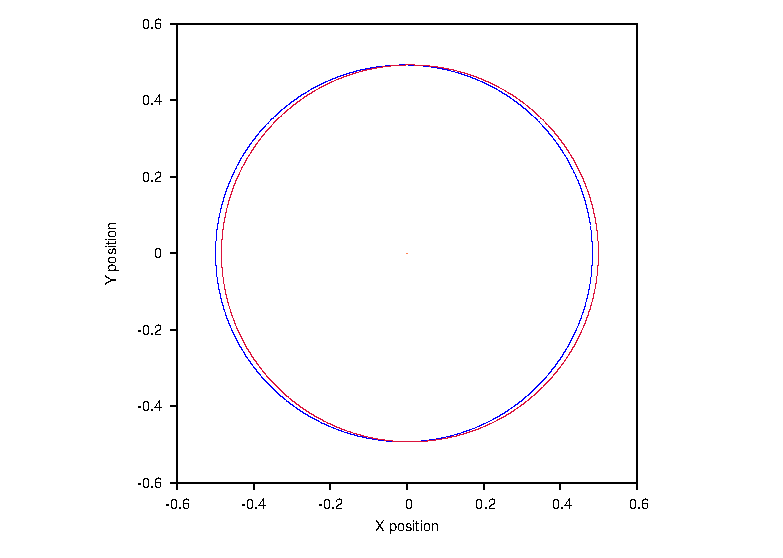
\includegraphics[width=.9\textwidth]{./2016results/stablebase/Orbit.eps}
\caption{Configuration 1}
\label{fig:config1}
\end{figure}

\begin{figure}[H]
\centering
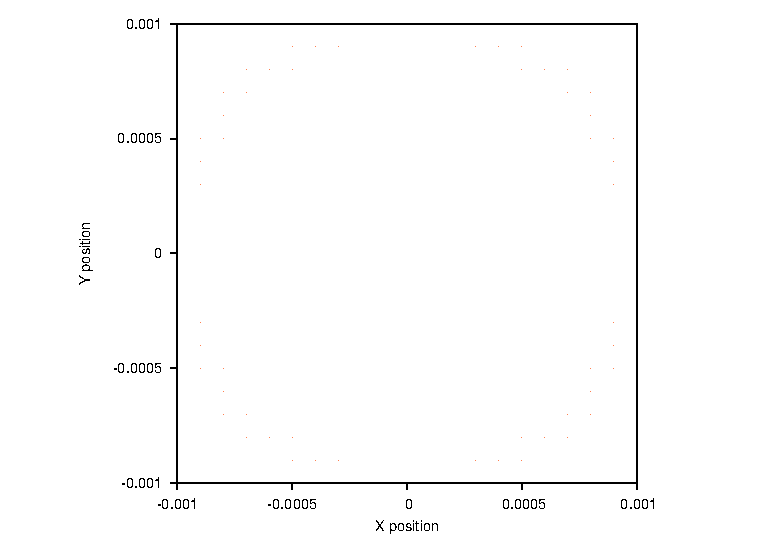
\includegraphics[width=.9\textwidth]{./2016results/stablebase/Inner.eps}
\caption{Configuration 1 - Inner Bar}
\label{fig:config1i}
\end{figure}

\begin{figure}[H]
\centering
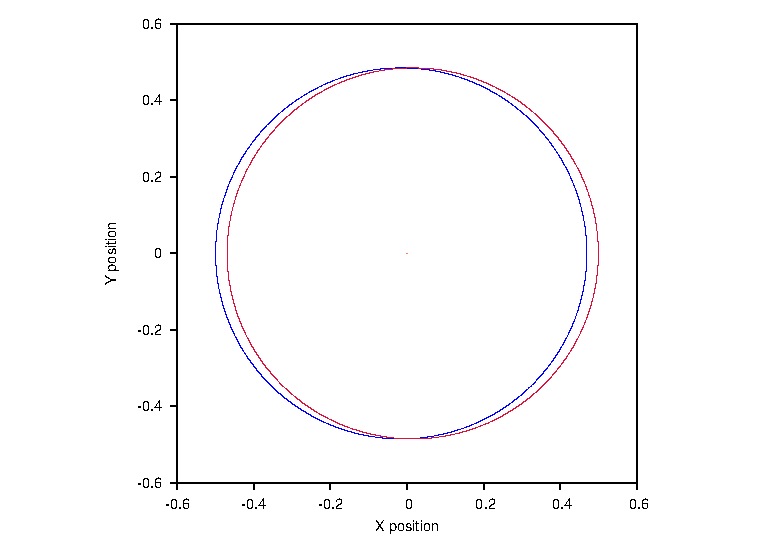
\includegraphics[width=.9\textwidth]{./2016results/002-5-001/Orbit.eps}
\caption{Configuration 2}
\label{fig:config2}
\end{figure}

\begin{figure}[H]
\centering
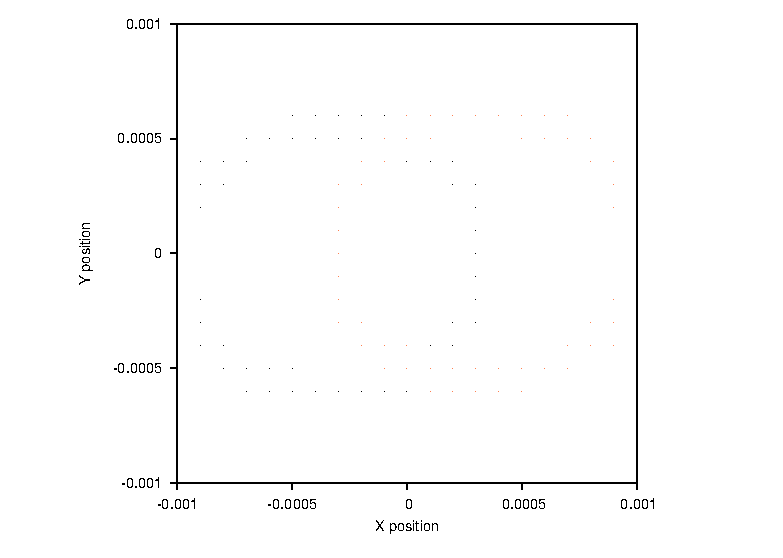
\includegraphics[width=.9\textwidth]{./2016results/002-5-001/Inner.eps}
\caption{Configuration 2 - Inner Bar}
\label{fig:config2i}
\end{figure}

\begin{figure}[H]
\centering
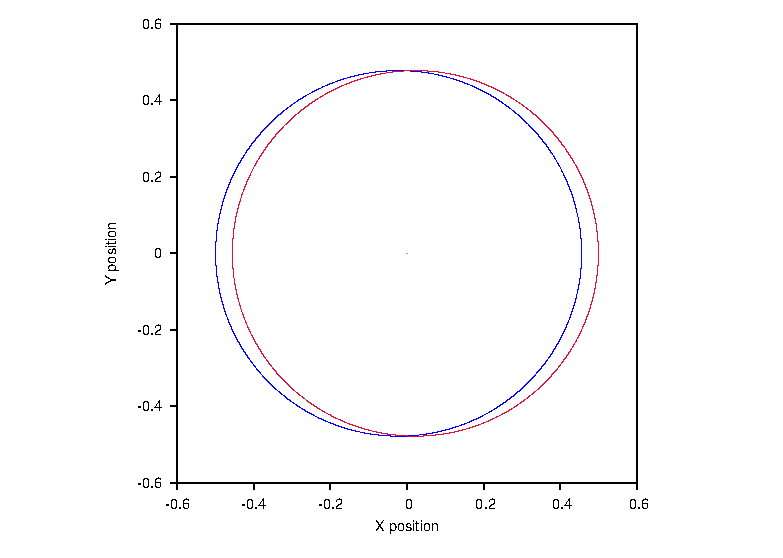
\includegraphics[width=.9\textwidth]{./2016results/003-5-001/Orbit.eps}
\caption{Configuration 3}
\label{fig:config3}
\end{figure}
\begin{figure}[H]
\centering
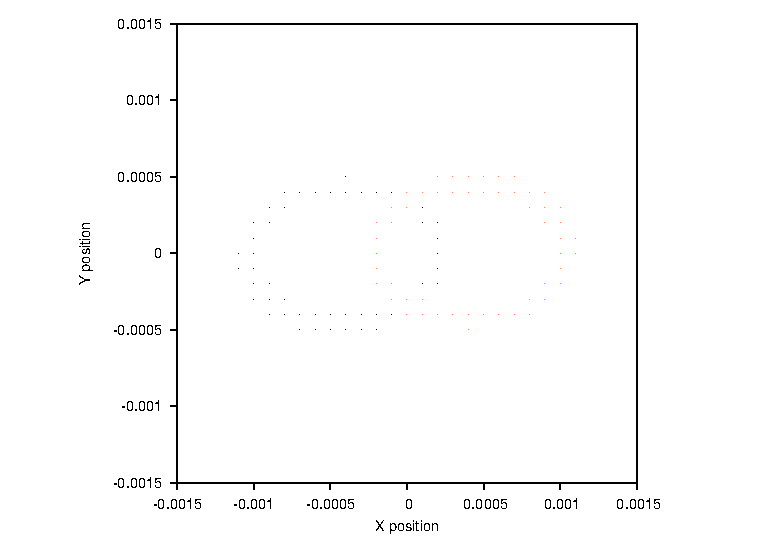
\includegraphics[width=.9\textwidth]{./2016results/003-5-001/Inner.eps}
\caption{Configuration 3 - Inner Bar}
\label{fig:config3i}
\end{figure}

\begin{figure}[H]
\centering
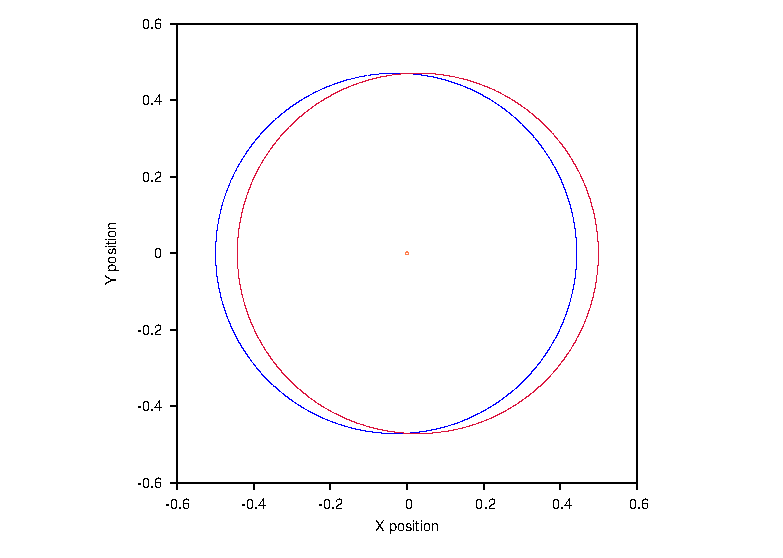
\includegraphics[width=0.9\textwidth]{./2016results/004-5-004/Orbit.eps}
\caption{Configuration 4}
\label{fig:config4}
\end{figure}
\begin{figure}[H]
\centering
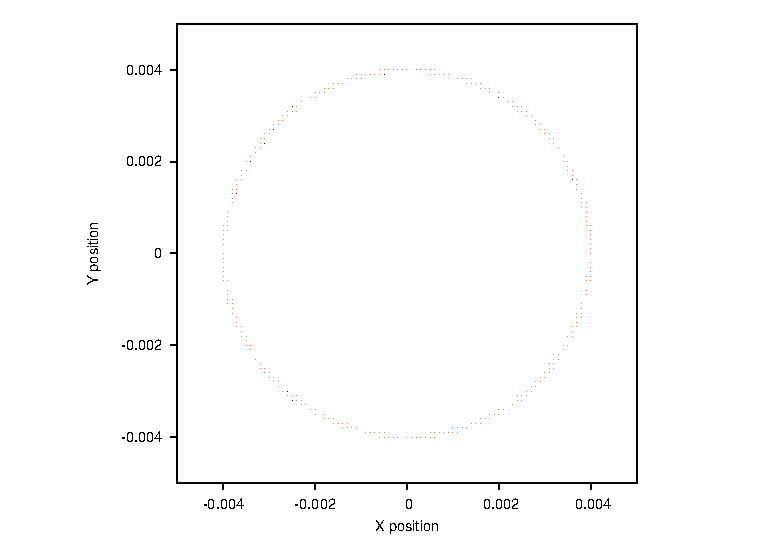
\includegraphics[width=0.9\textwidth]{./2016results/004-5-004/Inner.eps}
\caption{Configuration 4 - Inner Bar}
\label{fig:config4i}
\end{figure}

\begin{figure}[H]
\centering
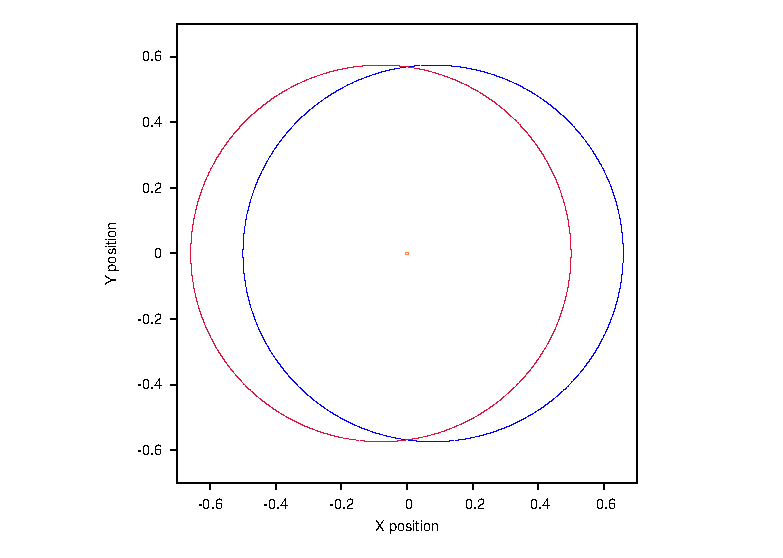
\includegraphics[width=0.9\textwidth]{./2016results/004-55-004/Orbit.eps}
\caption{Configuration 5}
\label{fig:config5}
\end{figure}
\begin{figure}[H]
\centering
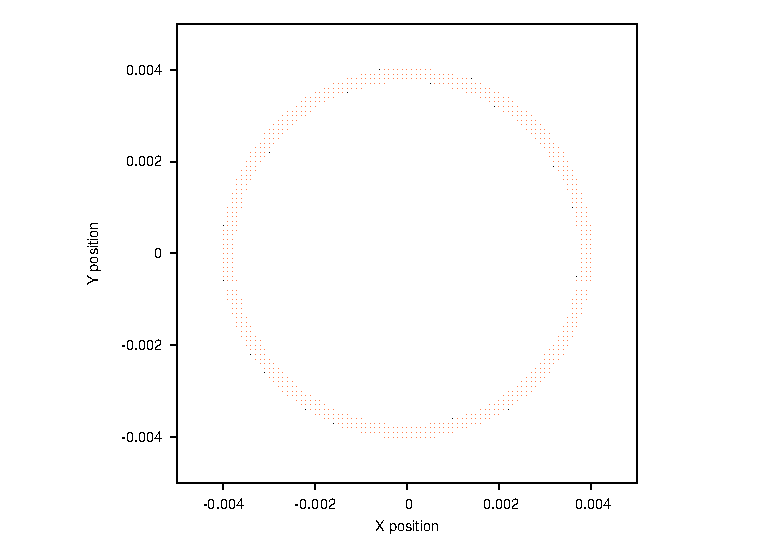
\includegraphics[width=0.9\textwidth]{./2016results/004-55-004/Inner.eps}
\caption{Configuration 5 - Inner Bar}
\label{fig:config5i}
\end{figure}

\begin{figure}[H]
\centering
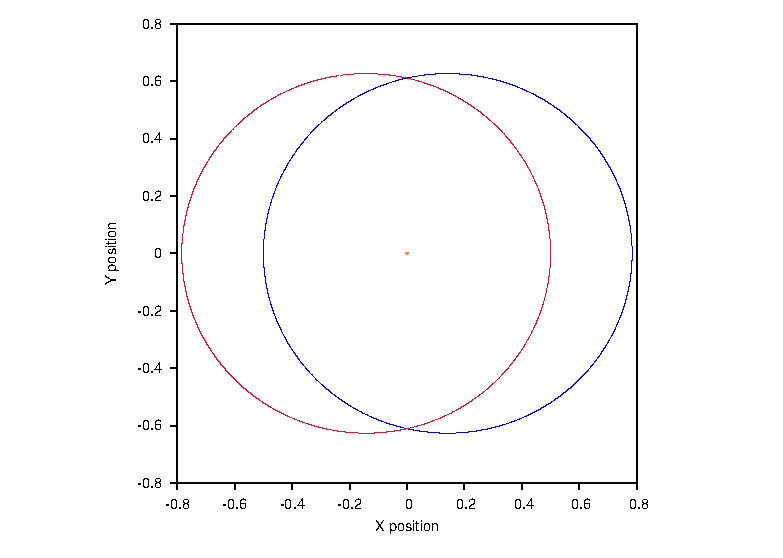
\includegraphics[width=0.9\textwidth]{./2016results/004-57-004/Orbit.eps}
\caption{Configuration 6}
\label{fig:config6}
\end{figure}
\begin{figure}[H]
\centering
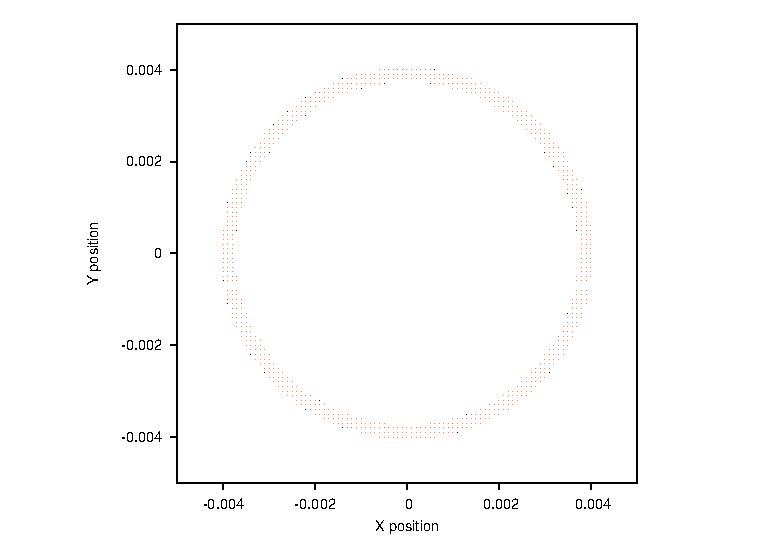
\includegraphics[width=0.9\textwidth]{./2016results/004-57-004/Inner.eps}
\caption{Configuration 6 - Inner Bar}
\label{fig:config6i}
\end{figure}

\begin{figure}[H]
\centering
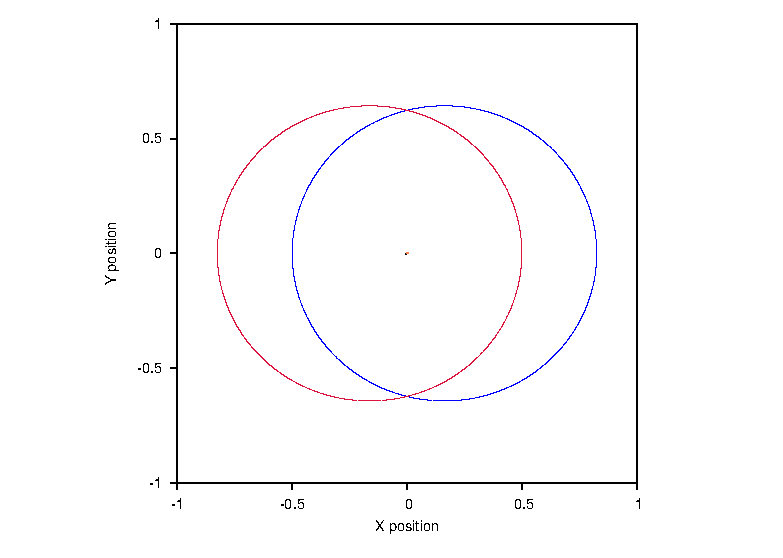
\includegraphics[width=0.9\textwidth]{./2016results/005-58-005-3/Orbit.eps}
\caption{Configuration 7}
\label{fig:config7}
\end{figure}
\begin{figure}[H]
\centering
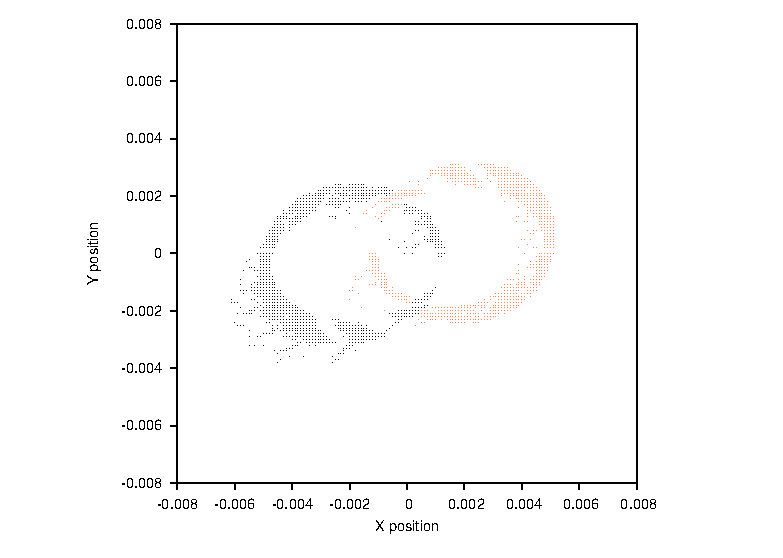
\includegraphics[width=0.9\textwidth]{./2016results/005-58-005-3/Inner.eps}
\caption{Configuration 7 - Inner Bar}
\label{fig:config7i}
\end{figure}

\begin{figure}[H]
\centering
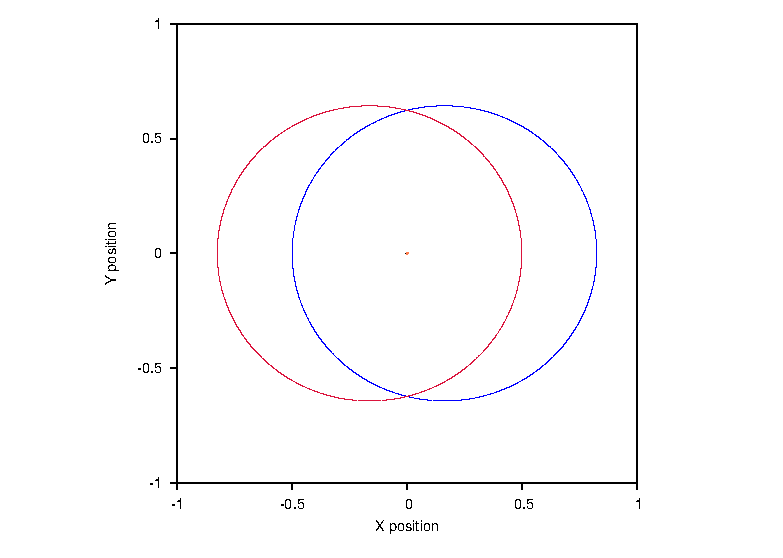
\includegraphics[width=0.9\textwidth]{./2016results/005-58-005-4/Orbit.eps}
\caption{Configuration 8}
\label{fig:config8}
\end{figure}
\begin{figure}[H]
\centering
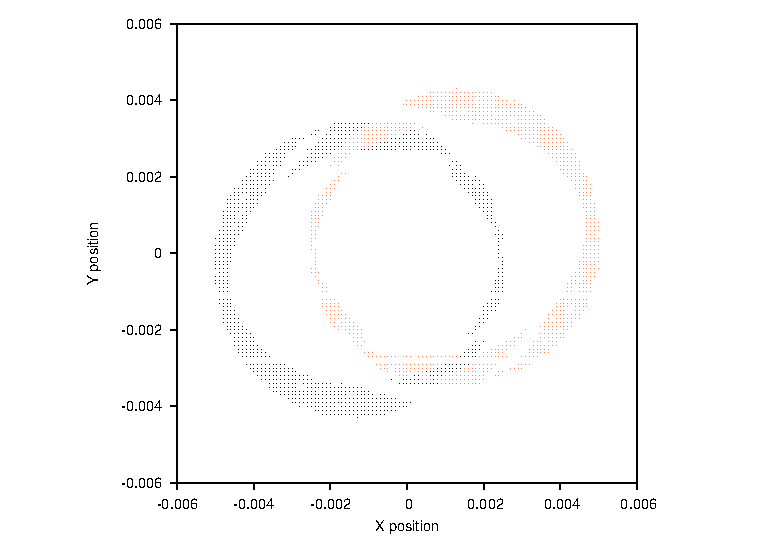
\includegraphics[width=0.9\textwidth]{./2016results/005-58-005-4/Inner.eps}
\caption{Configuration 8 - Inner Bar}
\label{fig:config8i}
\end{figure}

\begin{figure}[H]
\centering
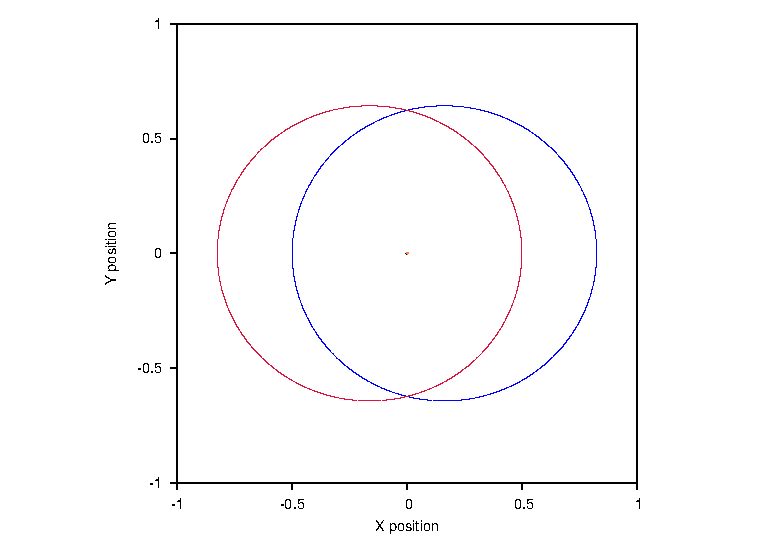
\includegraphics[width=0.9\textwidth]{./2016results/005-58-005-35/Orbit.eps}
\caption{Configuration 9}
\label{fig:config9}
\end{figure}
\begin{figure}[H]
\centering
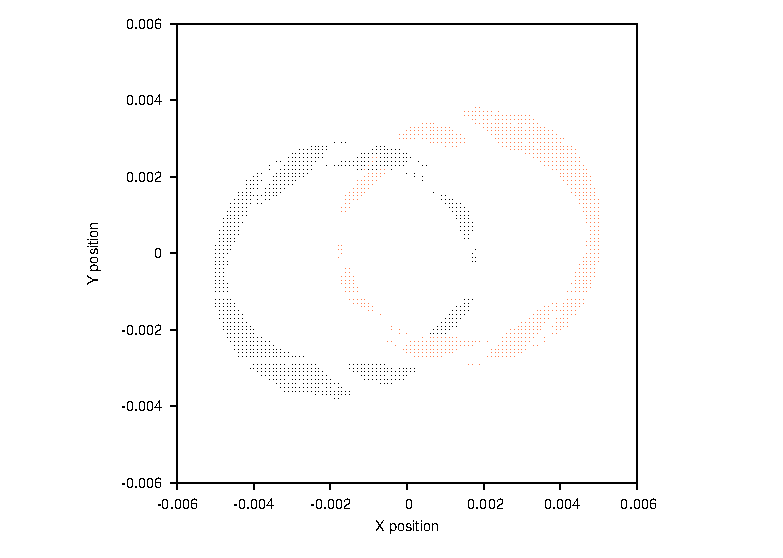
\includegraphics[width=0.9\textwidth]{./2016results/005-58-005-35/Inner.eps}
\caption{Configuration 9 - Inner Bar}
\label{fig:config9i}
\end{figure}

\begin{figure}[H]
\centering
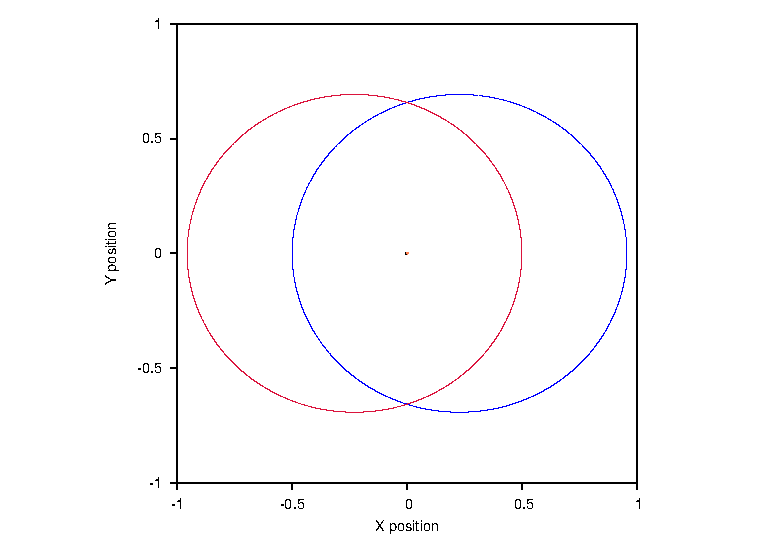
\includegraphics[width=0.9\textwidth]{./2016results/006-6-006-3/Orbit.eps}
\caption{Configuration 10}
\label{fig:config10}
\end{figure}
\begin{figure}[H]
\centering
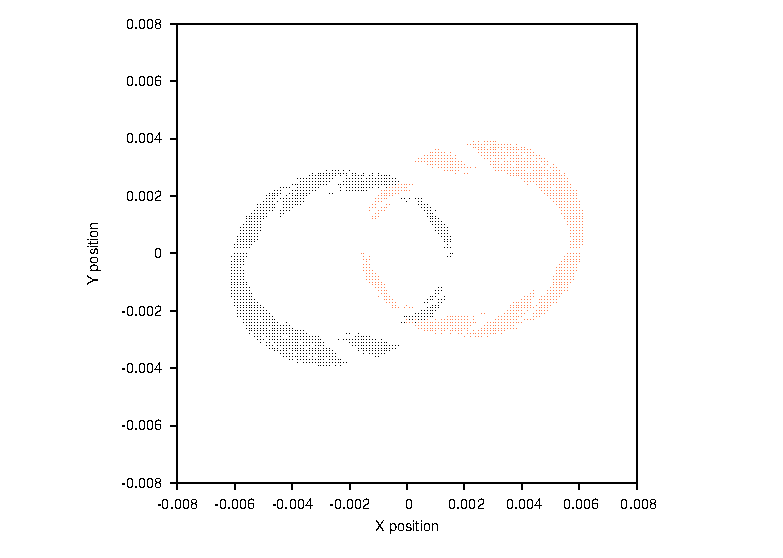
\includegraphics[width=0.9\textwidth]{./2016results/006-6-006-3/Inner.eps}
\caption{Configuration 10 - Inner Bar}
\label{fig:config10i}
\end{figure}

\begin{figure}[H]
\centering
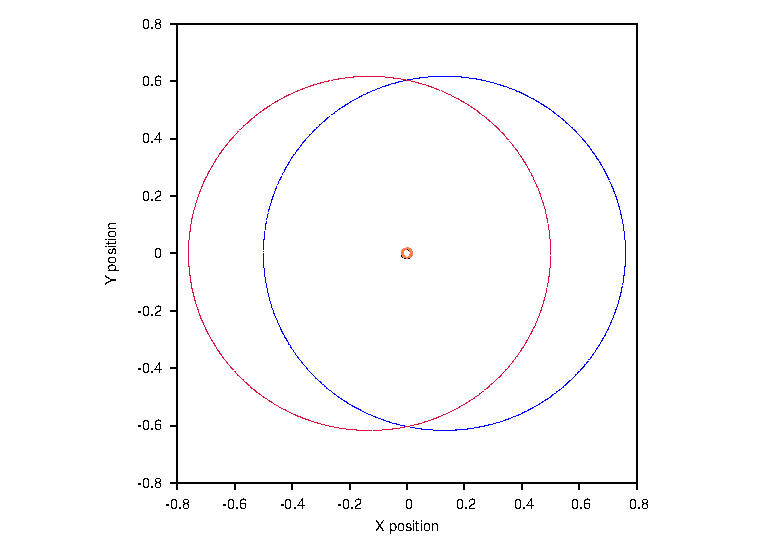
\includegraphics[width=0.9\textwidth]{./2016results/025-65-02/Orbit.eps}
\caption{Configuration 11}
\label{fig:config11}
\end{figure}
\begin{figure}[H]
\centering
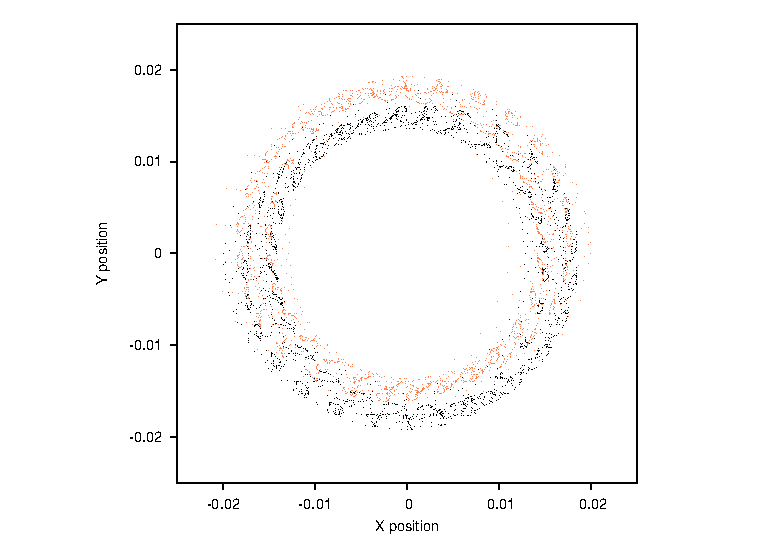
\includegraphics[width=0.9\textwidth]{./2016results/025-65-02/Inner.eps}
\caption{Configuration 11 - Inner Bar}
\label{fig:config11i}
\end{figure}

\begin{figure}[H]
\centering
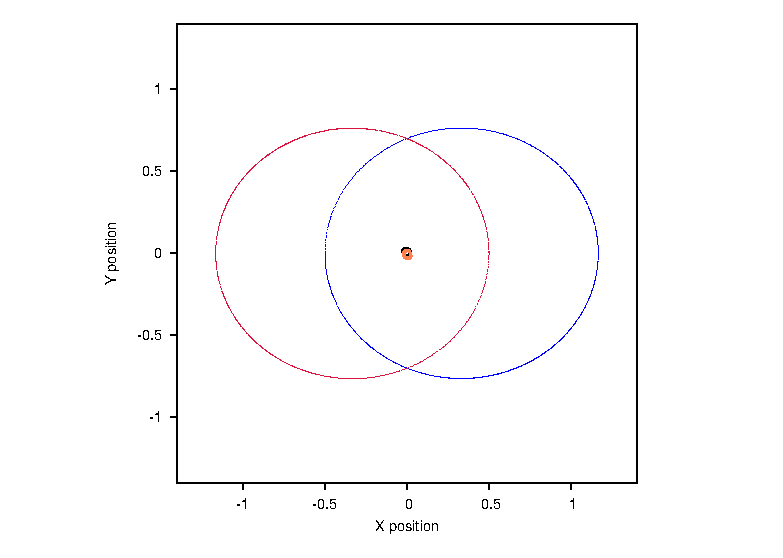
\includegraphics[width=0.9\textwidth]{./2017results/025-7-025-5/Orbit.eps}
\caption{Configuration 12}
\label{fig:config12}
\end{figure}
\begin{figure}[H]
\centering
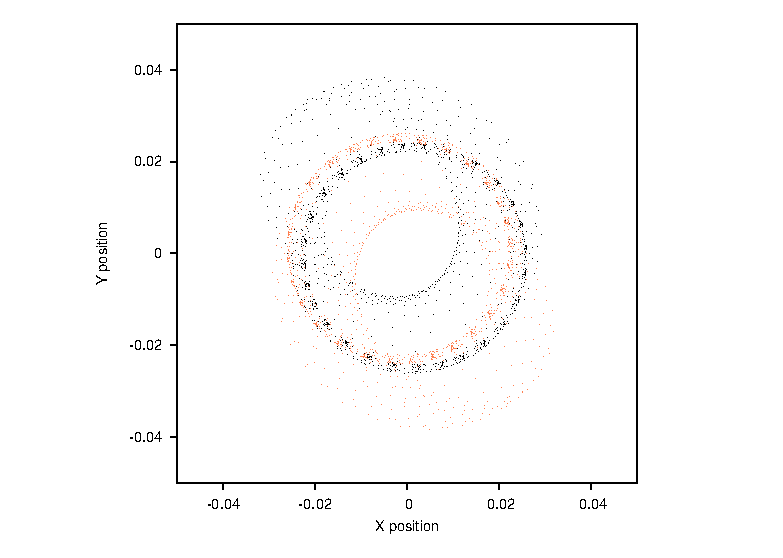
\includegraphics[width=0.9\textwidth]{./2017results/025-7-025-5/Inner.eps}
\caption{Configuration 12 - Inner Bar}
\label{fig:config12i}
\end{figure}

\begin{figure}[H]
\centering
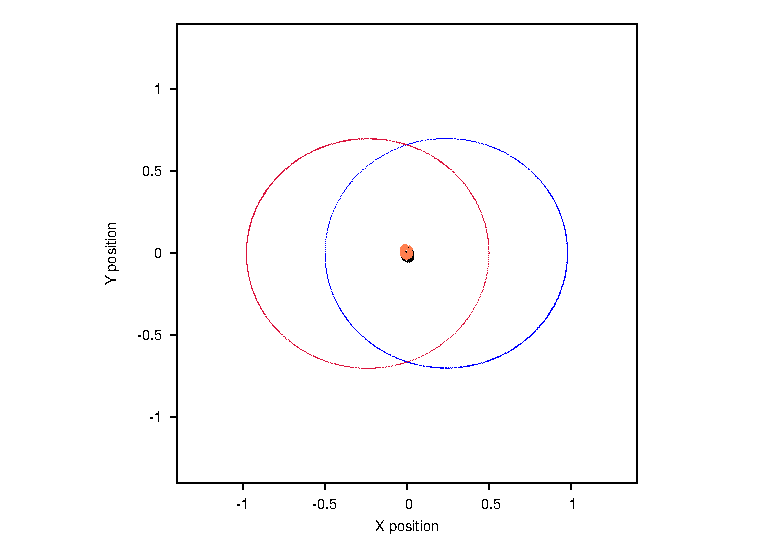
\includegraphics[width=0.9\textwidth]{./2017results/03-7-03-5/Orbit.eps}
\caption{Configuration 13}
\label{fig:config13}
\end{figure}
\begin{figure}[H]
\centering
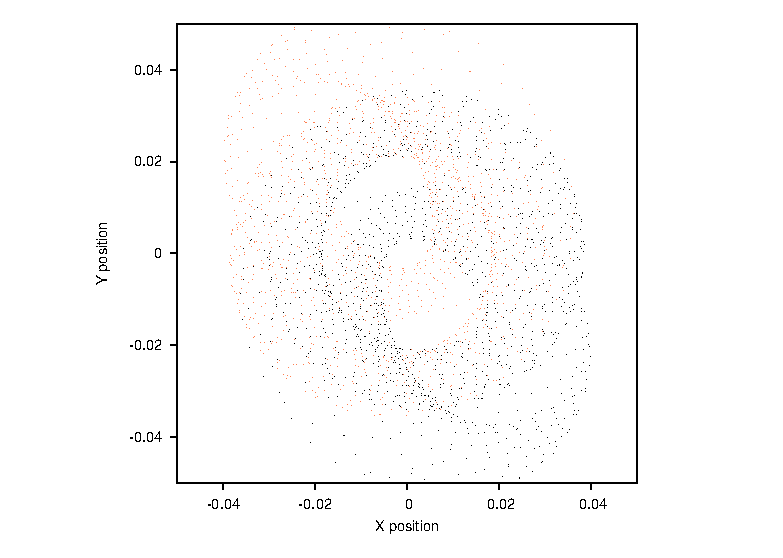
\includegraphics[width=0.9\textwidth]{./2017results/03-7-03-5/Inner.eps}
\caption{Configuration 13 - Inner Bar}
\label{fig:config13i}
\end{figure}

\begin{figure}[H]
\centering
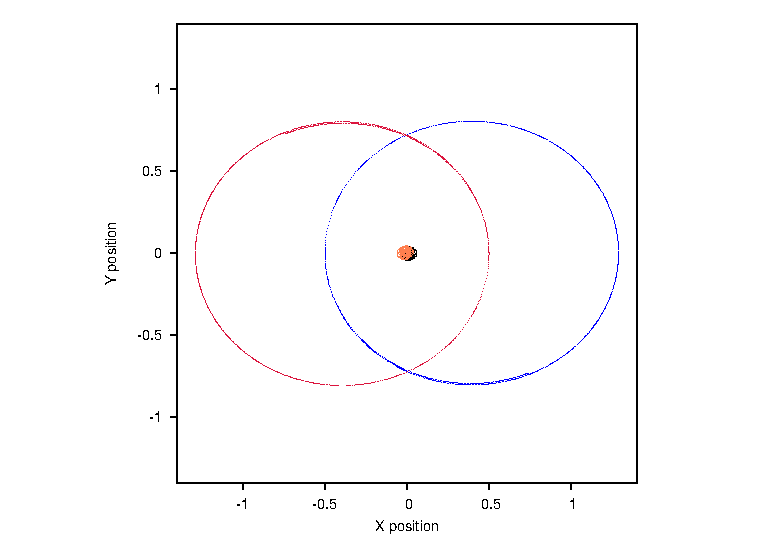
\includegraphics[width=0.9\textwidth]{./2017results/035-75-04-4/Orbit.eps}
\caption{Configuration 14}
\label{fig:config14}
\end{figure}
\begin{figure}[H]
\centering
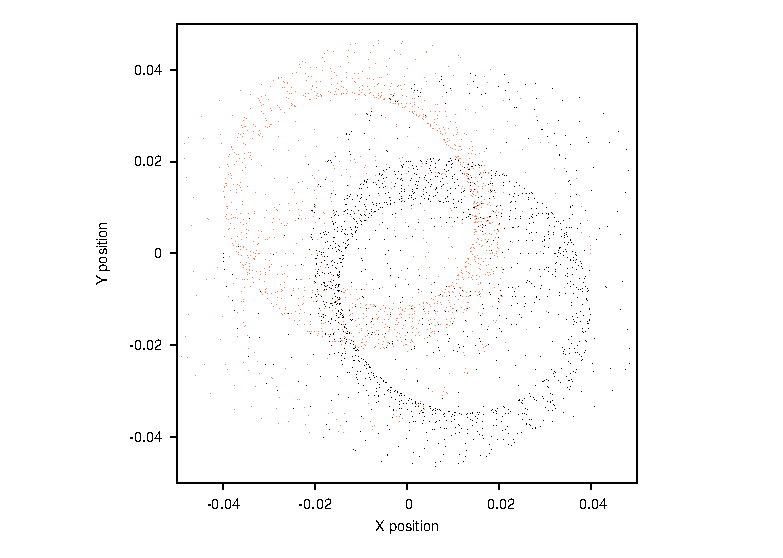
\includegraphics[width=0.9\textwidth]{./2017results/035-75-04-4/Inner.eps}
\caption{Configuration 14 - Inner Bar}
\label{fig:config14i}
\end{figure}

\begin{figure}[H]
\centering
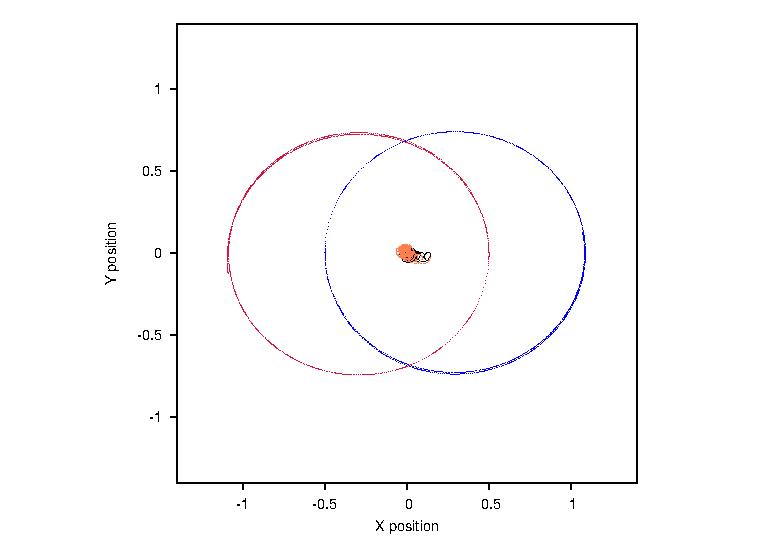
\includegraphics[width=0.9\textwidth]{./2017results/04-75-045-4/Orbit.eps}
\caption{Configuration 15}
\label{fig:config15}
\end{figure}
\begin{figure}[H]
\centering
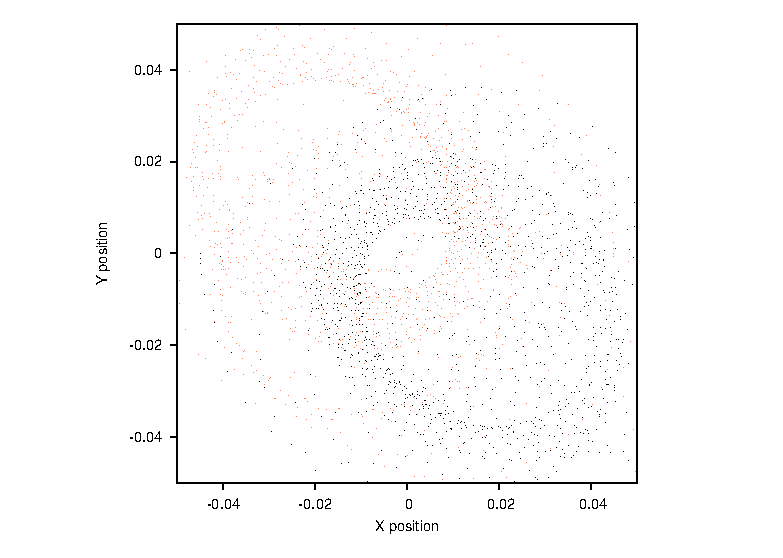
\includegraphics[width=0.9\textwidth]{./2017results/04-75-045-4/Inner.eps}
\caption{Configuration 15 - Inner Bar}
\label{fig:config15i}
\end{figure}

\begin{figure}[H]
\centering
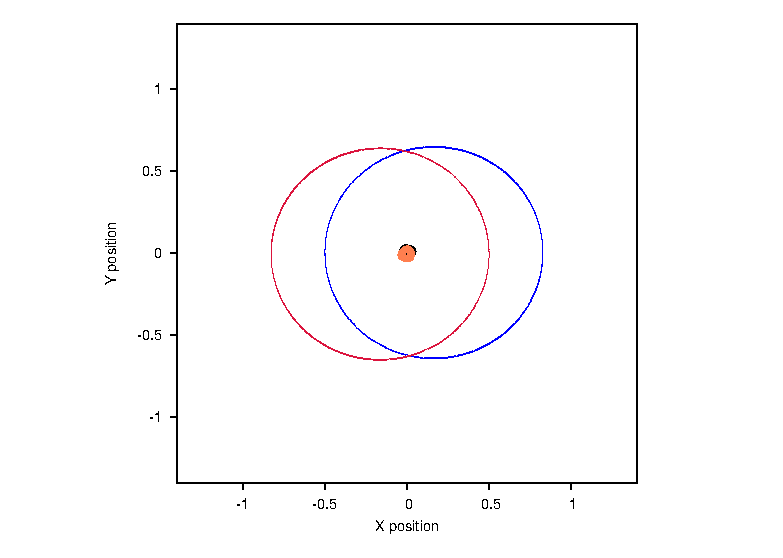
\includegraphics[width=0.9\textwidth]{./2017results/05-75-045-4/Orbit.eps}
\caption{Configuration 16}
\label{fig:config16}
\end{figure}
\begin{figure}[H]
\centering
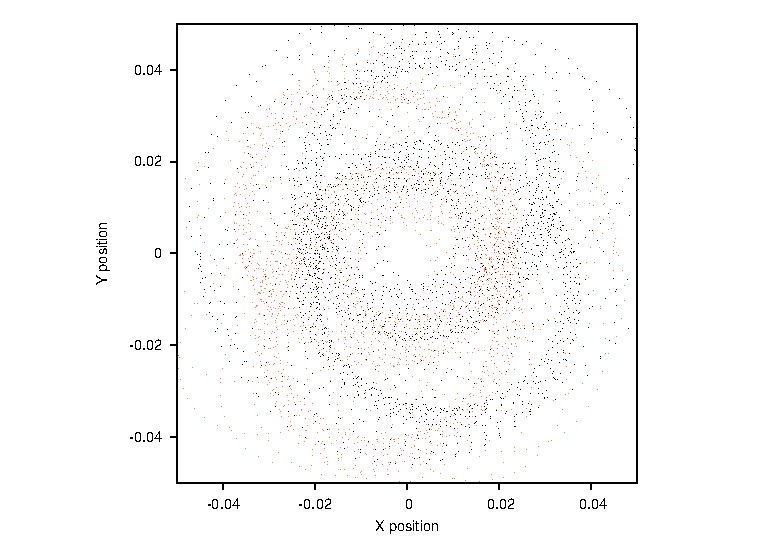
\includegraphics[width=0.9\textwidth]{./2017results/05-75-045-4/Inner.eps}
\caption{Configuration 16 - Inner Bar}
\label{fig:config16i}
\end{figure}

\begin{figure}[H]
\centering
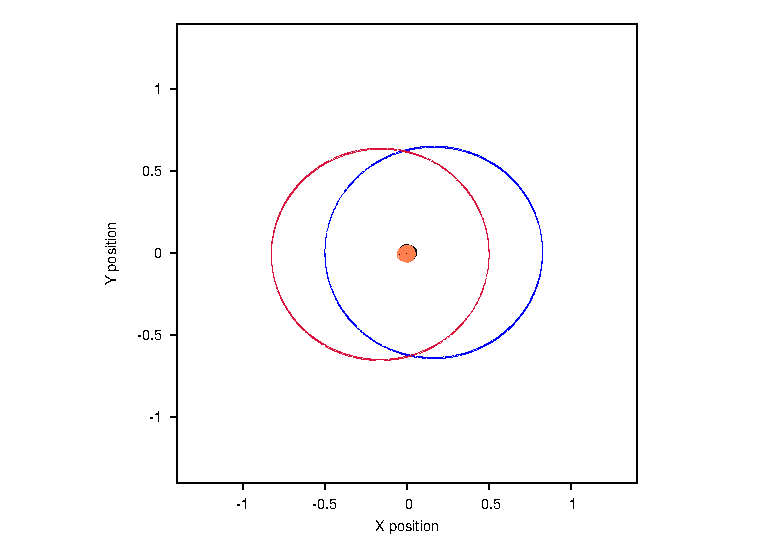
\includegraphics[width=0.9\textwidth]{./2017results/05-75-05-35/Orbit.eps}
\caption{Configuration 17}
\label{fig:config17}
\end{figure}
\begin{figure}[H]
\centering
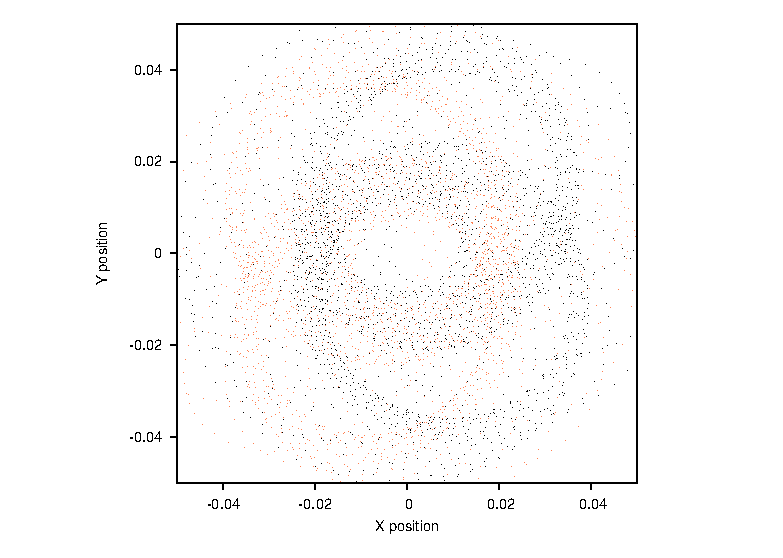
\includegraphics[width=0.9\textwidth]{./2017results/05-75-05-35/Inner.eps}
\caption{Configuration 17 - Inner Bar}
\label{fig:config17i}
\end{figure}

\begin{figure}[H]
\centering
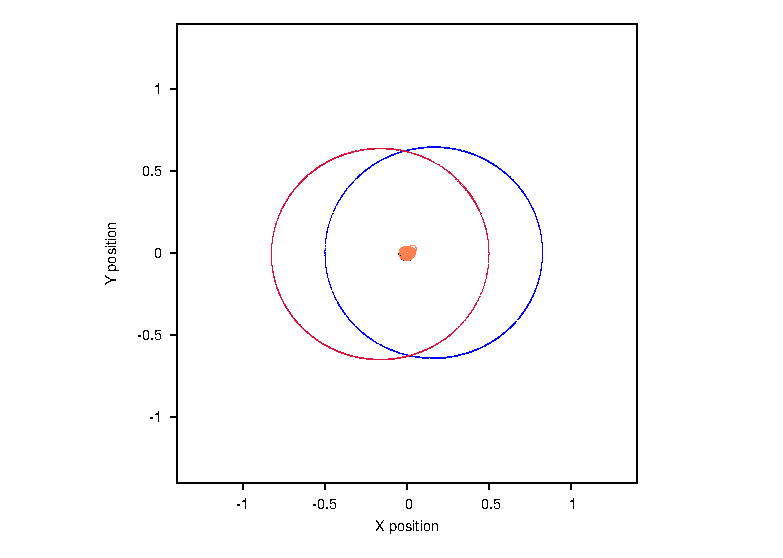
\includegraphics[width=0.9\textwidth]{./2017results/05-75-05-3/Orbit.eps}
\caption{Configuration 18}
\label{fig:config18}
\end{figure}
\begin{figure}[H]
\centering
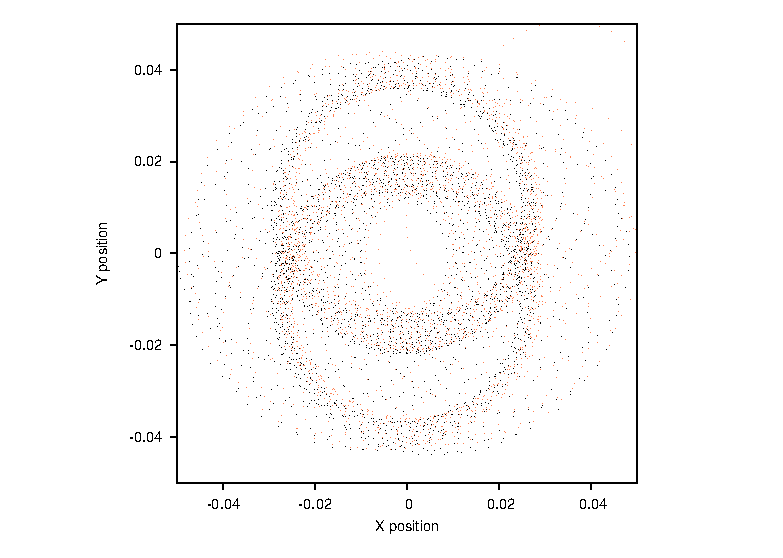
\includegraphics[width=0.9\textwidth]{./2017results/05-75-05-3/Inner.eps}
\caption{Configuration 18 - Inner Bar}
\label{fig:config18i}
\end{figure}

\begin{figure}[H]
\centering
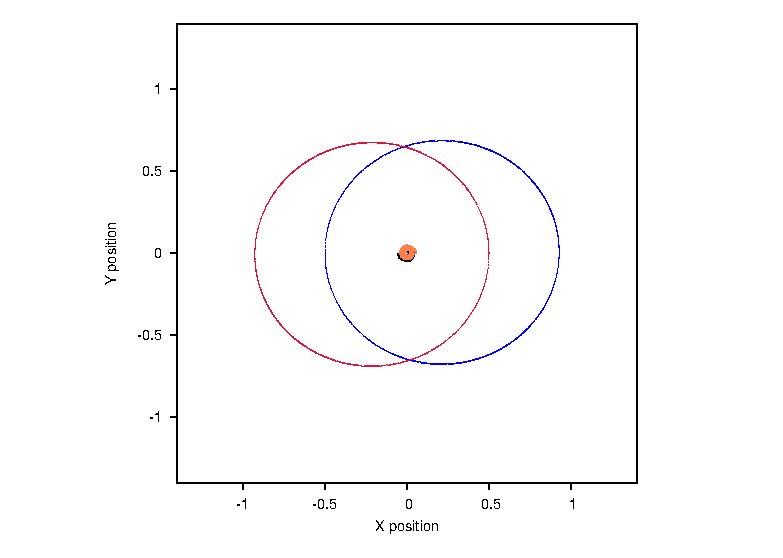
\includegraphics[width=0.9\textwidth]{./2017results/06-8-06-25/Orbit.eps}
\caption{Configuration 19}
\label{fig:config19}
\end{figure}
\begin{figure}[H]
\centering
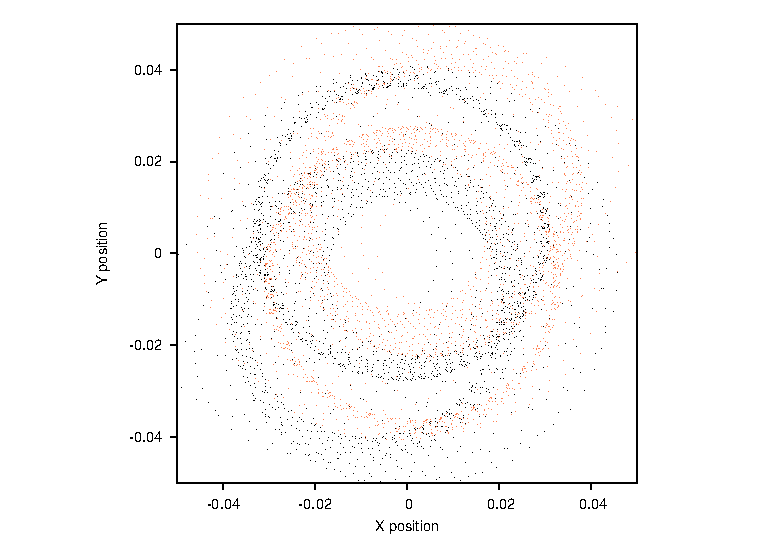
\includegraphics[width=0.9\textwidth]{./2017results/06-8-06-25/Inner.eps}
\caption{Configuration 19 - Inner Bar}
\label{fig:config19i}
\end{figure}

\begin{figure}[H]
\centering
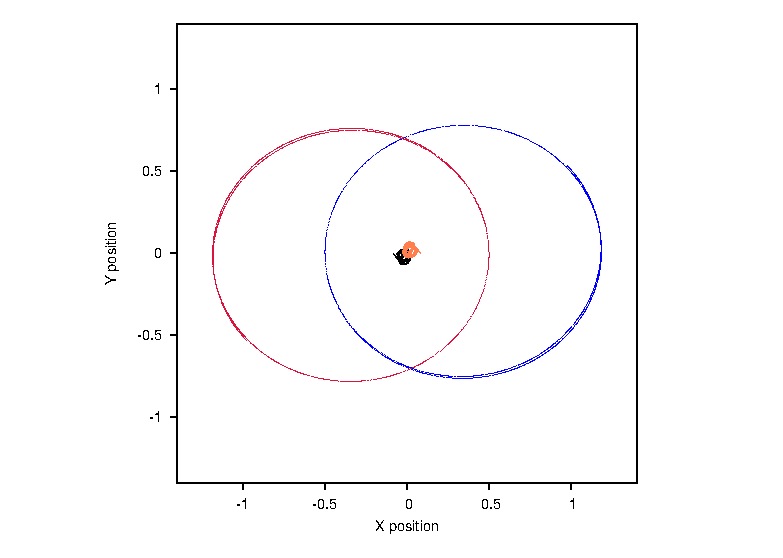
\includegraphics[width=0.9\textwidth]{./2017results/08-9-08-15/Orbit.eps}
\caption{Configuration 20}
\label{fig:config20}
\end{figure}
\begin{figure}[H]
\centering
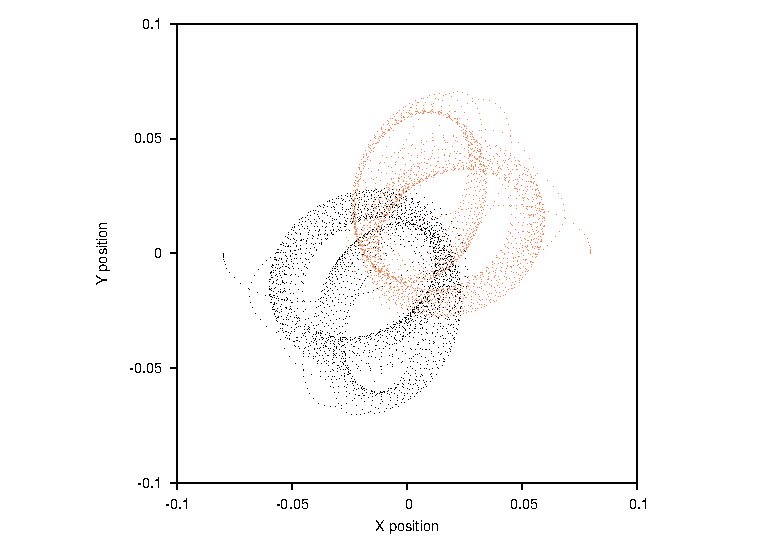
\includegraphics[width=0.9\textwidth]{./2017results/08-9-08-15/Inner.eps}
\caption{Configuration 20 - Inner Bar}
\label{fig:config20i}
\end{figure}

\begin{figure}[H]
\centering
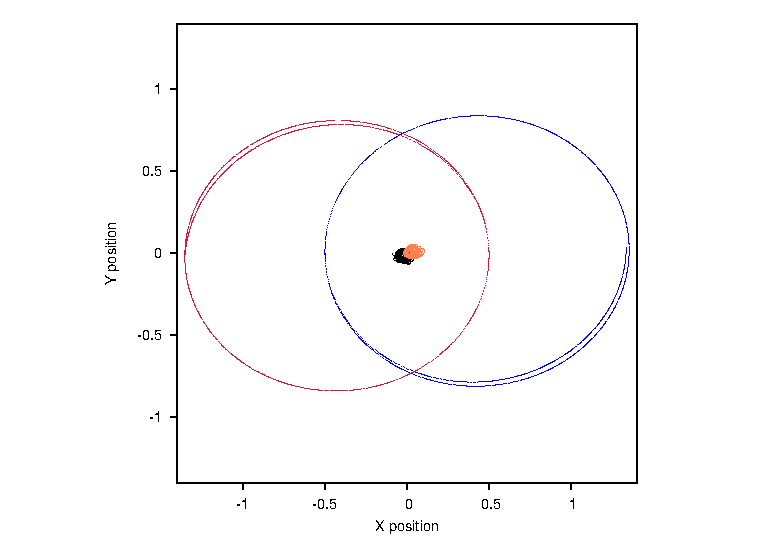
\includegraphics[width=0.9\textwidth]{./2017results/09-95-09-1/Orbit.eps}
\caption{Configuration 21}
\label{fig:config21}
\end{figure}
\begin{figure}[H]
\centering
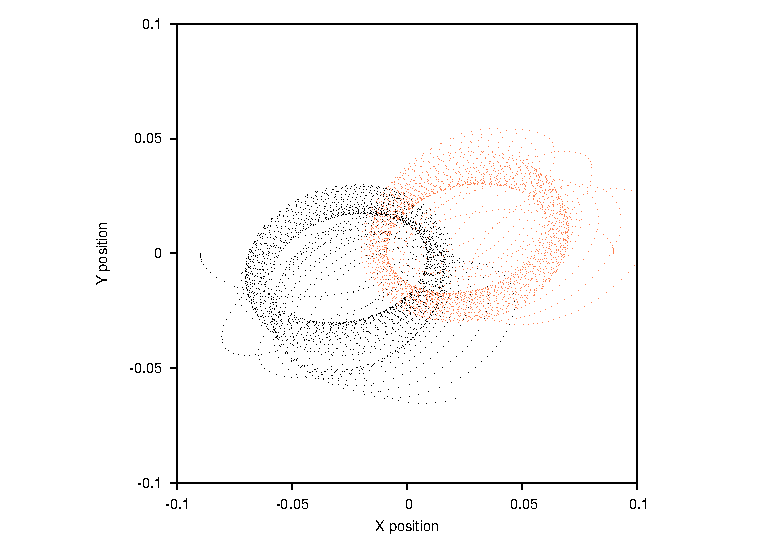
\includegraphics[width=0.9\textwidth]{./2017results/09-95-09-1/Inner.eps}
\caption{Configuration 21 - Inner Bar}
\label{fig:config21i}
\end{figure}

\begin{figure}[H]
\centering
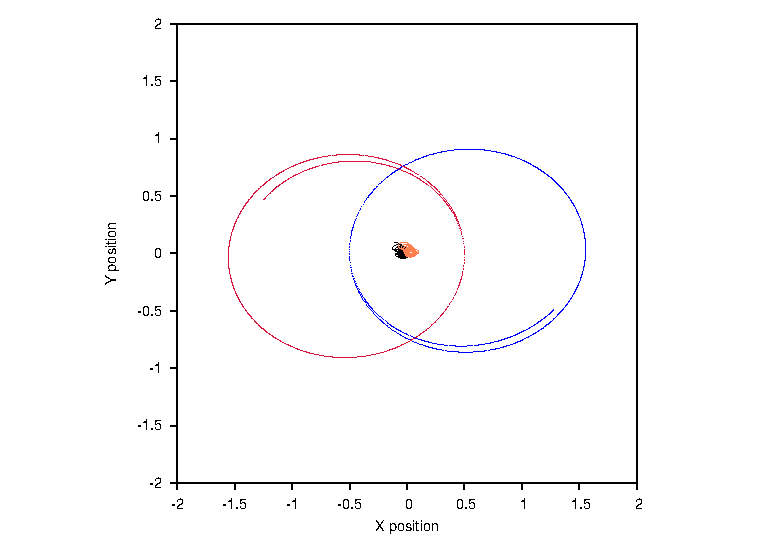
\includegraphics[width=0.9\textwidth]{./2017results/1-1-1-05/Orbit.eps}
\caption{Configuration 22}
\label{fig:config22}
\end{figure}
\begin{figure}[H]
\centering
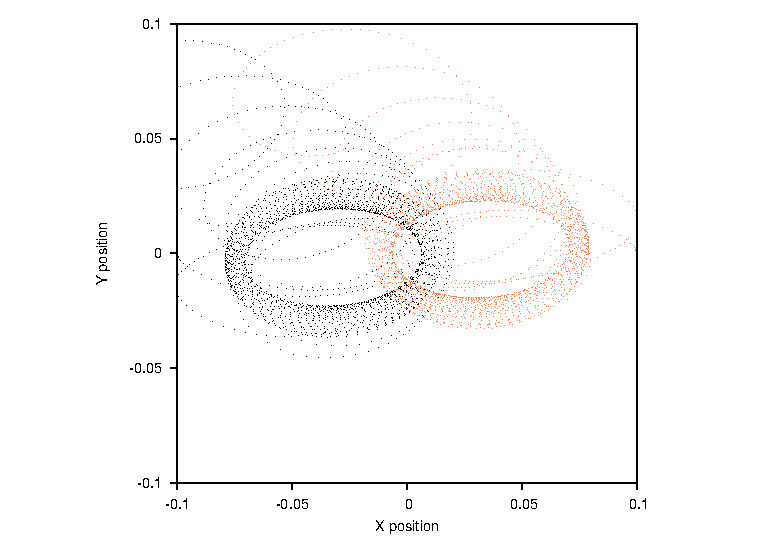
\includegraphics[width=0.9\textwidth]{./2017results/1-1-1-05/Inner.eps}
\caption{Configuration 22 - Inner Bar}
\label{fig:config22i}
\end{figure}

\begin{figure}[H]
\centering
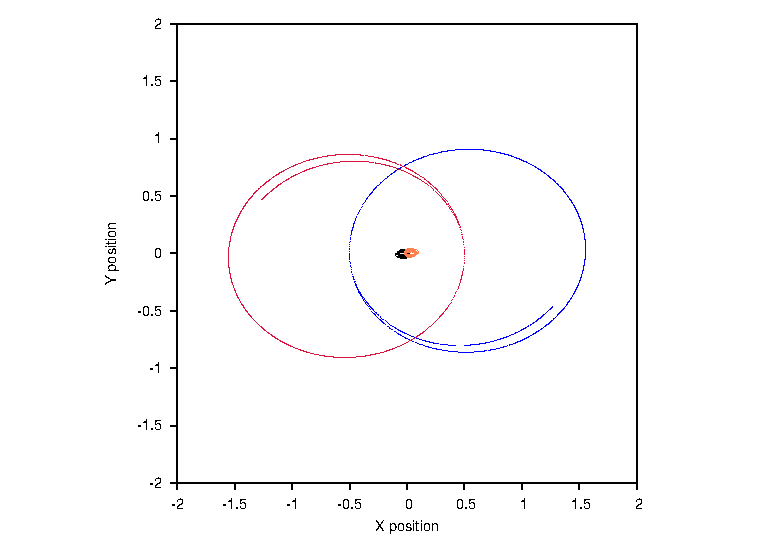
\includegraphics[width=0.9\textwidth]{./2017results/1-1-1-04/Orbit.eps}
\caption{Configuration 23}
\label{fig:config23}
\end{figure}
\begin{figure}[H]
\centering
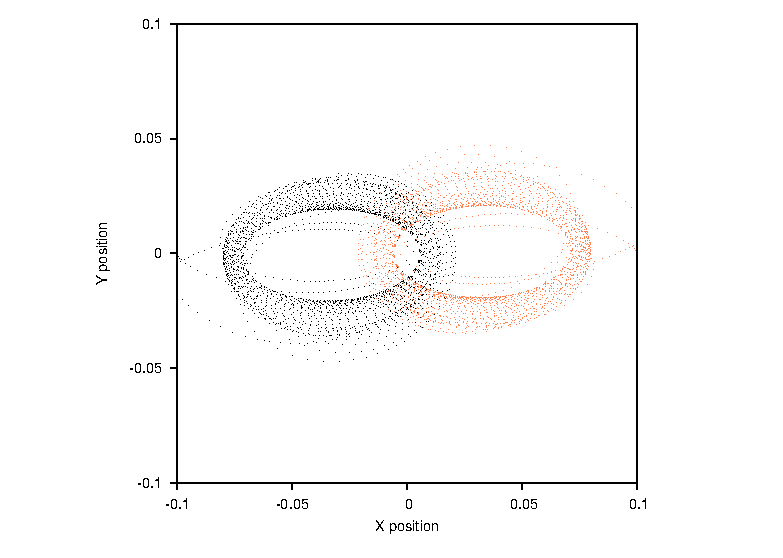
\includegraphics[width=0.9\textwidth]{./2017results/1-1-1-04/Inner.eps}
\caption{Configuration 23 - Inner Bar}
\label{fig:config23i}
\end{figure}

\begin{figure}[H]
\centering
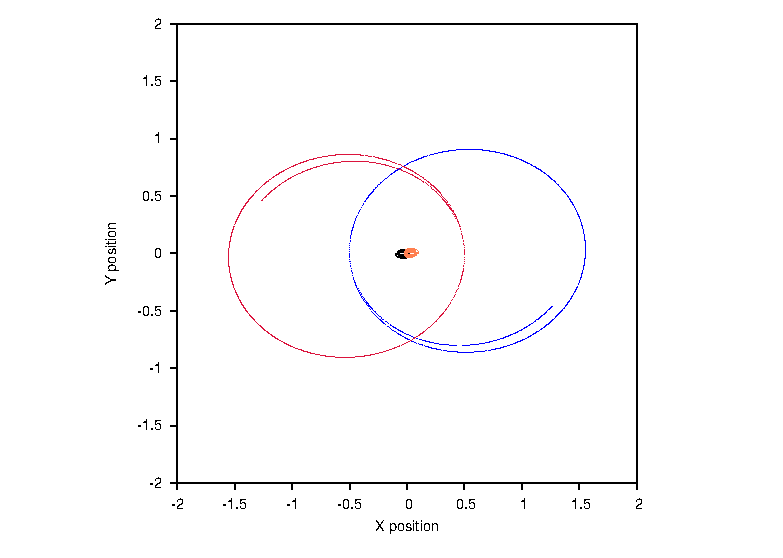
\includegraphics[width=0.9\textwidth]{./2017results/1-1-1-03/Orbit.eps}
\caption{Configuration 24}
\label{fig:config24}
\end{figure}
\begin{figure}[H]
\centering
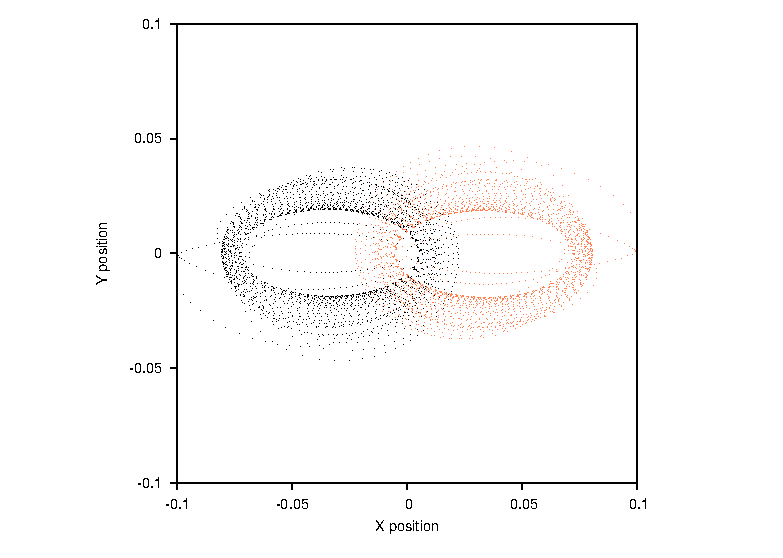
\includegraphics[width=0.9\textwidth]{./2017results/1-1-1-03/Inner.eps}
\caption{Configuration 24 - Inner Bar}
\label{fig:config24i}
\end{figure}

\begin{figure}[H]
\centering
\includegraphics[width=0.9\textwidth]{./2017results/1-1-1-02/Orbit.eps}
\caption{Configuration 25}
\label{fig:config25}
\end{figure}
\begin{figure}[H]
\centering
\includegraphics[width=0.9\textwidth]{./2017results/1-1-1-02/Inner.eps}
\caption{Configuration 25 - Inner Bar}
\label{fig:config25i}
\end{figure}

\begin{figure}[H]
\centering
\includegraphics[width=0.9\textwidth]{./2017results/12-105-11-015/Orbit.eps}
\caption{Configuration 26}
\label{fig:config26}
\end{figure}
\begin{figure}[H]
\centering
\includegraphics[width=0.9\textwidth]{./2017results/12-105-11-015/Inner.eps}
\caption{Configuration 26 - Inner Bar}
\label{fig:config26i}
\end{figure}

\begin{figure}[H]
\centering
\includegraphics[width=0.9\textwidth]{./2017results/12-11-11-015/Orbit.eps}
\caption{Configuration 27}
\label{fig:config27}
\end{figure}
\begin{figure}[H]
\centering
\includegraphics[width=0.9\textwidth]{./2017results/12-11-11-015/Inner.eps}
\caption{Configuration 27 - Inner Bar}
\label{fig:config27i}
\end{figure}

\begin{figure}[H]
\centering
\includegraphics[width=0.9\textwidth]{./2017results/12-11-115-015/Orbit.eps}
\caption{Configuration 28}
\label{fig:config28}
\end{figure}
\begin{figure}[H]
\centering
\includegraphics[width=0.9\textwidth]{./2017results/12-11-115-015/Inner.eps}
\caption{Configuration 28 - Inner Bar}
\label{fig:config28i}
\end{figure}

\begin{figure}[H]
\centering
\includegraphics[width=0.9\textwidth]{./2017results/12-11-12-015/Orbit.eps}
\caption{Configuration 29}
\label{fig:config29}
\end{figure}
\begin{figure}[H]
\centering
\includegraphics[width=0.9\textwidth]{./2017results/12-11-12-015/Inner.eps}
\caption{Configuration 29 - Inner Bar}
\label{fig:config29i}
\end{figure}

\begin{figure}[H]
\centering
\includegraphics[width=0.9\textwidth]{./2017results/1-1-1-1/Orbit.eps}
\caption{Configuration 30}
\label{fig:config30}
\end{figure}
\begin{figure}[H]
\centering
\includegraphics[width=0.9\textwidth]{./2017results/1-1-1-1/Inner.eps}
\caption{Configuration 30 - Inner Bar}
\label{fig:config30i}
\end{figure}

\begin{thebibliography}{1}
\bibitem[Erwin(2008)]{erwin1}Erwin, P., Double-Barred Galaxies, 2008, Mem. S.A.It. Vol. 75, 282
\bibitem[Du et. al.(2015)]{du}Du, M., Shen, J., Debattista, V., Forming Double-Barred Galaxies from Dynamically Cool Inner Disks, 2015, The Astrophysical Journal, 804:139 (10pp), 2015 May 10
\bibitem[Wozniak(2015)]{wozniak}Wozniak, H., How can double-barred galaxies be long-lived?, 2015, A and A 575, A7 (2015)
\bibitem[Debattista and Shen(2007)]{debattista}Debattista, V., Shen, J., Long-Lived Double-Barred Galaxies from Psuedobulges, 2007, The Astrophysical Journal, 654: L127–L130, 2007 January 10
\bibitem[Garzon(2014)]{garzon}Garzon, F., Lopez-Corredoira, M., Dynamical evolution of two associated galactic bars, 2014, arXiv:1409.1916.v1
\bibitem[Alvarez–Ramirez and Medina(2014)]{alvarez}Alvarez–Ramirez, M., Medina, M., A Review of the Planar Caledonian Four-Body Problem, 2014, TODO
\bibitem[Szell et. al.(2004)]{szell}Szell, A., Erdi, B., Sandor, Zs., Steves, B., Chaotic and stable behaviour in the Caledonian Symmetric Four-Body Problem, 2004, Mon. Not. R. Astron. Soc. 347, 380Ð388 (2004)
\bibitem[Steves and Roy(1998)]{steves}Steves, B., Roy, A., Some special restricted four-body problems-I. Modelling the Caledonian problem, 1998, Phrt. Spucx, Si., Vol. 46. No. I I /) 12, pp. 1465-1474, 1998
\bibitem[Shen and Debattista(2009)]{shen}Shen, J., Debattista, V., Observable Properties of Double-Barred Galaxies in N-Body Simulations, 2009, The Astrophysical Journal, 690:758–772, 2009 January 1
\bibitem[Erwin and Sparke(2002)]{erwin2}Erwin, P., Sparke, L., Double Bars, Inner Disks, and Nuclear Rings in Early-Type Disk Galaxies, 2002, The Astronomical Journal, 124:65–77, 2002 July
\bibitem[Binney and Tremaine(2008)]{binney}Binney, J., Tremaine, S., Galactic Dynamics, 2008, Princeton University Press
\bibitem[Aarseth(2003)]{aarseth}Aarseth, S., Gravitational N-Body Simulations, 2003, Cambridge University Press
\bibitem[Heggie and Hut(2002)]{heggie}Heggie D., Hut, P., The Gravitational Million-Body Problem, 2002, TODO
\bibitem[Erwin(2011)]{erwin3}Erwin, P., Double-Barred Galaxies, 2011, Mem. S.A.It. Suppl. Vol. 18, 145
\bibitem[Maciejewski(2003)]{macie1}Maciejewski, W., Chaos or Order in Double Barred Galaxies?, 2003, arXiv:astro-ph/0304432v1
\bibitem[Maciejewski and Athanassoula(2008)]{macie1}Maciejewski, W., Athanassoula, A., Regular motions in double bars. II. Survey of trajectories and 23 models, 2008, arXiv:0805.3967v1
\bibitem[Maciejewski and Small(2010)]{macie2}Maciejewski, W., Small, E., Orbital Support of Fast and Slow Inner Bars in Double Barred Galaxies, 2010, arXiv:1006.4574v1
\bibitem[Maciejewski and Sparke(1998)]{macie3}Maciejewski, W., Sparke, L., Bars within Bars in Galaxies, 1998, arXiv:astro-ph/9812228v1
\bibitem[Maciejewski and Sparke(1999)]{macie4}Maciejewski, W., Sparke, L., Orbits Supporting Bars within Bars, 1999, arXiv:astro-ph/9911281v1
\bibitem[Moulton(1914)]{moulton}Moulton, F., An Introduction to Celestial Mechanics, 1914, Palmyrin Library TODO
\bibitem[Trenti and Hut(2008)]{trenti}Trenti, M., Hut, P., Gravitational N-body Simulations, 2008, arXiv:0806.3950v1
\bibitem[Malhotra(1998)]{malhotra}Malhotra, R., Orbital Resonances and Chaos in the Solar System, 1998, Solar system Formation and Evolution ASP Conference Series, Vol. 149, 1998
\bibitem[Manos and Athanassoula(2011)]{manos}Manos, T., Athanassoula, E., Regular and chaotic orbits in barred galaxies - I. Applying the SALI/GALI method to explore their distribution in several models, 2011, arXiv:1102.1157v2
\bibitem[Saha and Maciejewski(2013)]{saha}Saha, K., Maciejewski, W., Spontaneous formation of double bars in dark matter dominated galaxies, 2013, arXiv:1304.7108v1
\bibitem[Sellwood and Wilkinson(2006)]{sellwood}Sellwood, J., Wilkinson, A., Dynamics of Barred Galaxies, 2006, arXiv:astro-ph/0608665v1
\bibitem[Collins(2004)]{collins}Collins, G., The Foundations Of Celestial Mechanics, 2004, Pachart Publishing House TODO
\end{thebibliography}
\end{document}